% Shared preamble for the repository diagrams. Each figure is compiled twice by build.sh: once as is
% (light theme) and once with \darktheme defined, which swaps the palette for a dark background.
\documentclass[tikz,border=4pt]{standalone}
\usepackage[T1]{fontenc}
\usepackage{lmodern}
\renewcommand{\familydefault}{\sfdefault}
\usepackage{amsmath,amssymb}
\usepackage{sansmath}
\sansmath
% Narrow boxes read better with whole words than with hyphenated ones.
\hyphenpenalty=10000
\exhyphenpenalty=10000
\usetikzlibrary{arrows.meta,positioning,calc,shapes.misc}

% Fill colors encode the role of a step: amber = test or rule, teal = forward simulation,
% purple = optimization or candidate generation, green = state or returned action, red = adverse
% outcome, blue = other processing.
\ifdefined\darktheme
  \definecolor{ink}{HTML}{E6EDF3}
  \definecolor{edge}{HTML}{8B949E}
  \definecolor{blue}{HTML}{1B2E45}
  \definecolor{teal}{HTML}{153C39}
  \definecolor{green}{HTML}{1C3823}
  \definecolor{amber}{HTML}{3F3313}
  \definecolor{red}{HTML}{442022}
  \definecolor{purple}{HTML}{30264A}
  \definecolor{grey}{HTML}{262B30}
  \definecolor{yes}{HTML}{56D364}
  \definecolor{no}{HTML}{F47067}
\else
  \definecolor{ink}{HTML}{17202A}
  \definecolor{edge}{HTML}{5D6670}
  \definecolor{blue}{HTML}{DDEBF7}
  \definecolor{teal}{HTML}{DDF2EF}
  \definecolor{green}{HTML}{E4F2E5}
  \definecolor{amber}{HTML}{FFF0CC}
  \definecolor{red}{HTML}{F8DDDD}
  \definecolor{purple}{HTML}{EAE2F5}
  \definecolor{grey}{HTML}{ECEFF1}
  \definecolor{yes}{HTML}{236B3B}
  \definecolor{no}{HTML}{A33636}
\fi

\tikzset{
  every picture/.style={color=ink, font=\small},
  box/.style={draw=edge, rounded corners=3pt, align=center, inner sep=4pt,
              text width=#1, minimum height=12mm, text=ink},
  box/.default=2.7cm,
  proc/.style={box=#1, fill=blue},   proc/.default=2.7cm,
  sim/.style={box=#1, fill=teal},    sim/.default=2.7cm,
  opt/.style={box=#1, fill=purple},  opt/.default=2.7cm,
  out/.style={box=#1, fill=green},   out/.default=2.7cm,
  bad/.style={box=#1, fill=red},     bad/.default=2.7cm,
  rule/.style={box=#1, fill=amber},  rule/.default=2.7cm,
  ask/.style={box=#1, fill=amber, chamfered rectangle, chamfered rectangle xsep=2pt,
              rounded corners=0pt, line width=0.6pt},
  ask/.default=2.7cm,
  arr/.style={-{Latex[length=2mm]}, semithick, draw=edge},
  darr/.style={arr, dashed},
  lab/.style={font=\scriptsize\bfseries, inner sep=1.5pt},
  ylab/.style={lab, text=yes}, nlab/.style={lab, text=no},
  note/.style={font=\scriptsize, text=ink, align=center},
}

\begin{document}
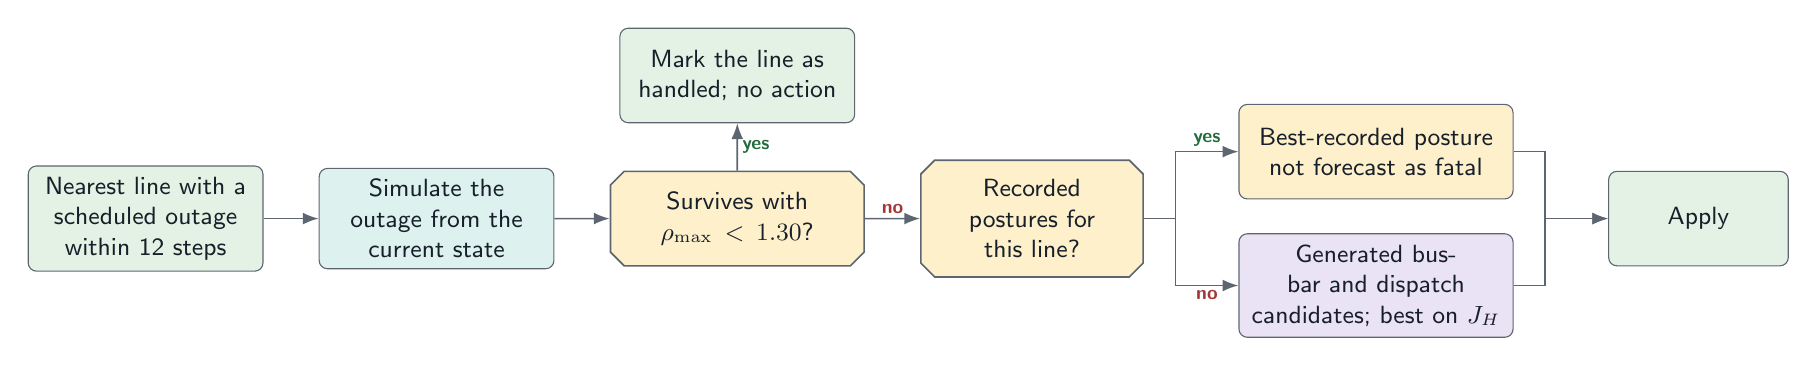
\begin{tikzpicture}[node distance=4mm and 7mm]
\node[out=2.7cm] (d) {Nearest line with a scheduled outage within 12 steps};
\node[sim, right=of d] (s) {Simulate the outage from the current state};
\node[ask=2.8cm, right=of s] (q) {Survives with $\rho_{\max}<1.30$?};
\node[out=2.7cm, above=6mm of q] (h) {Mark the line as handled; no action};
\node[ask=2.4cm, right=of q] (r) {Recorded postures for this line?};
\node[rule=3.2cm, right=12mm of r, yshift=8.5mm] (t) {Best-recorded posture not forecast as fatal};
\node[opt=3.2cm, right=12mm of r, yshift=-8.5mm] (g) {Generated bus-bar and dispatch candidates; best on $J_H$};
\node[out=2.0cm, right=12mm of t, yshift=-8.5mm] (a) {Apply};
\draw[arr] (d)--(s); \draw[arr] (s)--(q);
\draw[arr] (q)--node[ylab,right]{yes}(h);
\draw[arr] (q)--node[nlab,above]{no}(r);
\draw[arr] (r.east) -- ++(4mm,0) |- node[ylab,above,pos=0.75]{yes} (t.west);
\draw[arr] (r.east) -- ++(4mm,0) |- node[nlab,below,pos=0.75]{no} (g.west);
\draw[arr] (t.east) -- ++(4mm,0) |- (a.west);
\draw[arr] (g.east) -- ++(4mm,0) |- (a.west);
\end{tikzpicture}
\end{document}
